\clearpage
\section{Preparing the Game}

\begin{lessonbox}
Set up every unit listed in \rulesref{15.1--15.2}. The choices below specify
only the locations that matter to the tutorial. Units not named individually
may occupy any legal Objective Display in their assigned Zone; keep
\textbf{Pančevo} and \textbf{Cetinje} free of Axis units.
\end{lessonbox}

\begin{multicols}{2}
\small
\subsection{Key Axis Placements}

\rowcolors{2}{TitoBlue!42}{white}
\begin{tabularx}{\linewidth}{@{}>{\bfseries}l X@{}}
  \rowcolor{TitoInk!15}
  Unit & Objective Display \\
  German 704 & Belgrade \\
  German 714 & Kragujevac \\
  German 717 & Niš \\
  German 718 & Sarajevo \\
  Serbian 1--5 & Belgrade \\
  Italian Bergamo & Zagreb \\
  Italian Sassari & Karlovac \\
  Italian Macerata & Padgorica \\
\end{tabularx}
\rowcolors{2}{}{}

Place the remaining Italians throughout their assigned Zones, but leave
Cetinje empty. Place the Bulgarian 14th, 22nd, and 24th Divisions in Skopje,
Prilep, and Monastir respectively.

\subsection{Yugoslav Placements}

Place five Chetnik groups in the Serbia Chetnik Hide-away and two in the
Montenegro Chetnik Hide-away. All seven begin pro-Yugoslav.

\subsection{AGO Limit}

For this example, the Axis Player draws the Soviet counter with
\textbf{8 AGO} on its reverse. Keep it concealed as normal
\rulesref{15.31--15.32}. The example will expend three operations by the end
of Game-Turn 5.

\columnbreak

\subsection{Why This Setup?}

The starting deployments preserve the historical spheres of influence while
creating two safe Yugoslav probes:

\begin{itemize}[leftmargin=1.2em,itemsep=2pt]
  \item Pančevo offers the Chetniks a useful Recruitment Value of 1 and a
    Victory Point Value of 2.
  \item Cetinje offers a smaller but initially unopposed foothold.
  \item The German divisions remain close enough to demonstrate the Axis
    three-Zone movement allowance and a mandatory Objective combat.
  \item Croatia and Bosnia remain under-garrisoned, setting up the first
    uprising checks on Game-Turn 3.
\end{itemize}

\begin{commentarybox}
The original setup rules assign units to Zones, not to particular Objective
Displays. This freedom is intentional: two legal games can begin with quite
different local situations.
\end{commentarybox}

\subsection{Starting Tracks}

\begin{tabularx}{\linewidth}{@{}>{\bfseries}l X@{}}
  Game-Turn & 1 \\
  Yugoslav VP & 0 \\
  Allied Progress & Not yet begun \\
  Weather & Normal \\
  Tito & Not yet on map \\
  Partisan strength & 0 groups \\
  Chetnik strength & 7 pro-Yugoslav groups \\
\end{tabularx}
\end{multicols}

\vfill
\begin{center}
  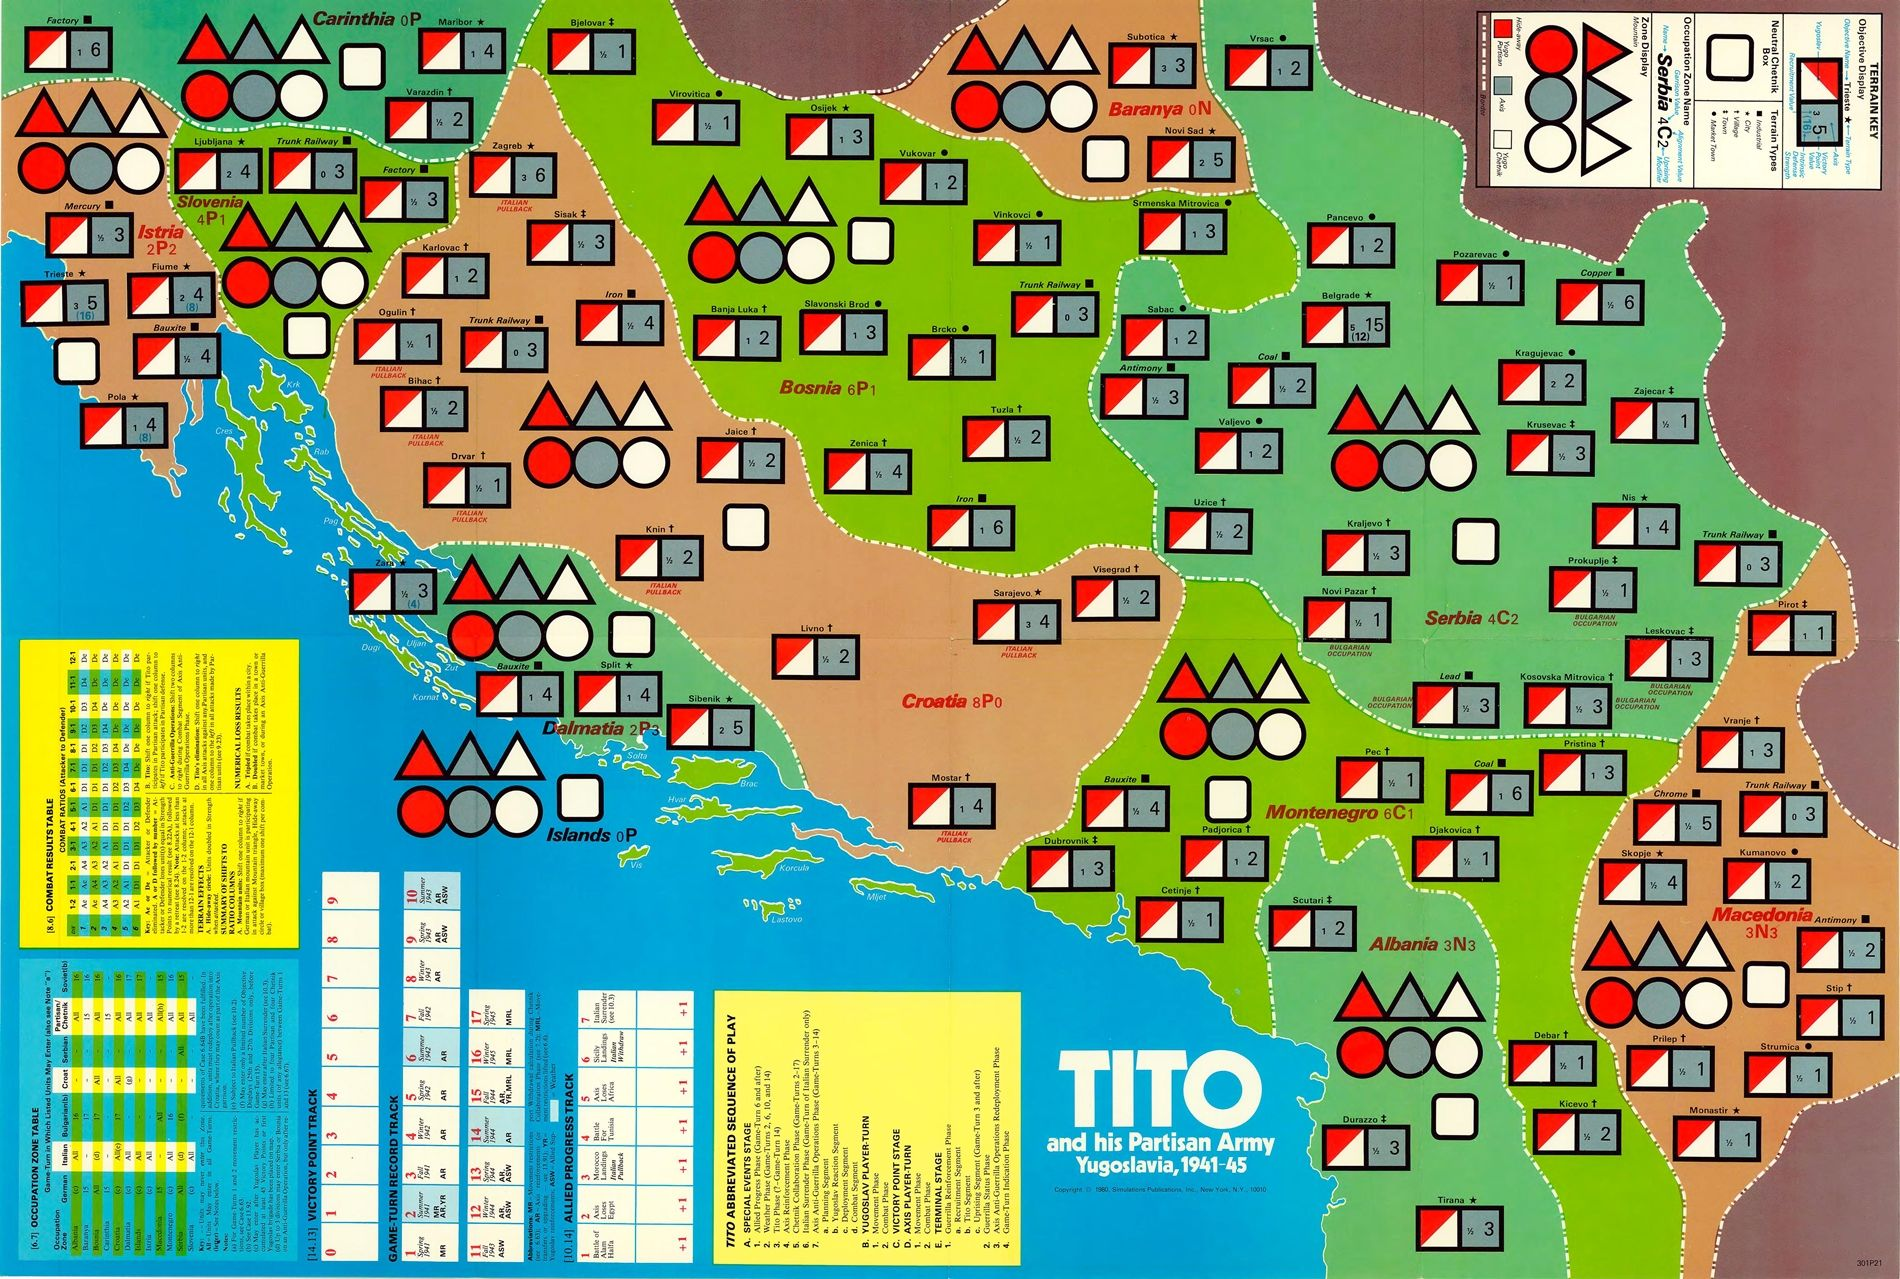
\includegraphics[width=0.67\linewidth,trim=70 120 40 70,clip]
    {../../Misc/Images/Tito/tito_map.jpg}
\end{center}

\begin{center}
\scriptsize\itshape
The full map before counters are placed. The tutorial’s opening action is
concentrated in Serbia and Montenegro; the conflict expands west on Turn 3.
\end{center}
